\documentclass{ieeeaccess}
\usepackage{cite}
\usepackage{amsmath,amssymb,amsfonts}
\usepackage{graphicx}
\usepackage{textcomp}
\usepackage{booktabs}
\usepackage{multirow}
\usepackage{array}
\usepackage[hidelinks]{hyperref}
\usepackage{url}
\urlstyle{same}
\newcommand{\MW}{\,\mathrm{MW}}
\newcommand{\CleanedPct}{0.07}
\newcommand{\MMGDfirst}{4--7\%}
\newcommand{\MMGDlast}{28--39\%}
\newcommand{\NHours}{130,128}


\begin{document}
\history{Date of publication xxxx 00, 0000, date of current version xxxx 00, 0000.}
\doi{10.1109/ACCESS.2026.DOI}

\title{Day-Ahead Load Forecasting for the Brazilian Interconnected Power System Under Rapid Distributed Solar Growth: An Open Benchmark Against the Operator's Official Forecast}

\author{\uppercase{Izialber Ozani Fernandes Muniz}\authorrefmark{1}}

\address[1]{Graduate Program in Production and Systems Engineering (PPPRO), Federal Center for Technological Education of Rio de Janeiro (CEFET/RJ), Rio de Janeiro, RJ 20271-110, Brazil}

\tfootnote{This work was supported in part by the Coordena\c{c}\~ao de Aperfei\c{c}oamento de Pessoal de N\'ivel Superior -- Brasil (CAPES) -- Finance Code 001.}

\markboth
{Muniz: Day-Ahead Load Forecasting for the Brazilian Interconnected Power System}
{Muniz: Day-Ahead Load Forecasting for the Brazilian Interconnected Power System}

\corresp{Corresponding author: Izialber Ozani Fernandes Muniz (e-mail: izialber.muniz@aluno.cefet-rj.br).}

\begin{abstract}
Rapid growth of behind-the-meter photovoltaic generation reshapes the load profile seen by transmission system operators, making day-ahead load forecasting a problem of persistent concept drift. Although open data now allow research models to be compared with the forecasts actually used in operation, such comparisons are rare. This paper presents an open and fully reproducible benchmark for day-ahead hourly load forecasting of the four subsystems of the Brazilian interconnected system, where behind-the-meter generation grew from about 5\% to one third of the midday load in five years. Using only public operator data (2012--2026), forecasts issued at noon of the previous day, and a test period of almost three years, we compare seasonal naive benchmarks, hour-specific linear autoregressive models, gradient boosting, a neural network, and their ensemble; study calibration windows and refitting frequencies; compare quantile regression with adaptive conformal prediction intervals; and evaluate the models against the operator's official day-ahead forecast. Without any weather input, the ensemble achieved a mean absolute percentage error of 2.44\%, versus 2.90\% for the official forecast, with significant improvements in three of the four subsystems according to Diebold--Mariano tests. The official forecast showed a systematic midday under-forecast that deepened from 2024 to 2026 as behind-the-meter generation grew, whereas the open models remained nearly unbiased. Level normalisation was essential for tree-based models, the calibration window mattered more than the refitting frequency, and adaptive conformal inference produced calibrated intervals where quantile gradient boosting was overconfident. Monitoring hour-specific bias and maintaining data-driven benchmarks can help operators cope with distributed solar growth.
\end{abstract}

\begin{keywords}
Load forecasting, behind-the-meter photovoltaics, concept drift, conformal prediction, gradient boosting, power system operation, Brazil.
\end{keywords}


\titlepgskip=-21pt

\maketitle

\section{Introduction}
\label{sec:introduction}

\PARstart{D}{ay-ahead} load forecasts are a central input of power system operation. Transmission system operators (TSOs) use them to schedule generation, set reserve requirements, and plan transmission constraints, so forecast errors translate directly into operating costs and security margins~\cite{hong2016tutorial,hong2020outlook}. Two developments are changing this task. First, the rapid diffusion of behind-the-meter photovoltaic (PV) generation makes the demand seen by the operator increasingly weather dependent and continuously reshapes the daily load profile, a persistent source of concept drift~\cite{gama2014drift}. Second, open data policies now give researchers access to the same measurements that operators use, which makes it possible to compare openly reproducible models with the forecasts actually used in operation, something rarely done in the load forecasting literature~\cite{hong2020outlook,petropoulos2022forecasting}.

These developments raise three practical questions that the literature does not answer jointly. (i) How accurate are open, data-driven day-ahead models, built only with information available at the operator's decision time, relative to the official forecast of a TSO? (ii) When load is drifting, how much history should be used to fit a model and how often should it be refitted? In electricity price forecasting, the choice and combination of calibration windows have been shown to matter~\cite{marcjasz2018windows,hubicka2019windows}, but for load this question has received little attention outside the abrupt COVID-19 shock~\cite{obst2021covid}. (iii) Can prediction intervals remain calibrated as the distribution of errors changes, for instance through adaptive conformal methods~\cite{gibbs2021aci,zaffran2022aci}?

We address these questions using a system that offers an unusually clear case of both developments. The Brazilian National Interconnected System (SIN) serves about 80~GW of average demand over a continental territory divided into four subsystems with distinct climates and consumption patterns. After the legal framework for distributed micro- and mini-generation (MMGD) was consolidated~\cite{lei14300}, behind-the-meter generation, mostly rooftop PV, grew from about 5\% of the midday load in 2021 to roughly one third in 2026, according to the operator's own estimates (Section~\ref{sec:data}). The National System Operator (ONS) publishes the hourly load of each subsystem since 2000, its MMGD estimates, and the official day-ahead load forecast used in the daily operation programming~\cite{ons_opendata,ons_apicarga}. The case therefore allows a long, fully reproducible evaluation against an operational reference, under a drift of a magnitude that other systems with fast PV adoption are likely to face.

The main contributions of this paper are as follows:
\begin{itemize}
\item We release an open and fully reproducible benchmark for day-ahead hourly load forecasting of the four SIN subsystems, built exclusively from public operator data (2012--2026), with an operationally realistic information set (forecasts issued at noon of the previous day, horizons of 14--37~h), a test period of almost three years never used for model design, and statistical significance testing.
\item We provide what is, to our knowledge, the first systematic comparison between open forecasting models and the official day-ahead forecast of a TSO under rapid behind-the-meter PV growth, including how the relative performance varies by hour of the day, by subsystem, and over time.
\item We quantify how the calibration window length (1 year to the full history) and the refitting frequency (daily to yearly) affect accuracy under drift, for linear and tree-based models, and show that a simple level normalisation of the target is decisive for tree ensembles.
\item We compare quantile gradient boosting, rolling empirical (split-conformal) intervals, and adaptive conformal inference with delayed feedback for day-ahead probabilistic load forecasting, and assess their calibration over time.
\item We analyse errors on special days (national holidays, Carnival, bridge days, and the year-end period), which are a major source of operational error in Brazil and many other countries~\cite{ziel2018holidays}.
\end{itemize}

The remainder of the paper is organised as follows. Section~\ref{sec:related} reviews related work. Section~\ref{sec:data} describes the data and Section~\ref{sec:method} the forecasting framework and evaluation protocol. Section~\ref{sec:results} presents the results, Section~\ref{sec:discussion} discusses their implications and limitations, and Section~\ref{sec:conclusion} concludes.

\section{Related Work}
\label{sec:related}

\subsection{Short-Term Load Forecasting Methods and Benchmarks}
Short-term load forecasting (STLF) has a long history in power systems. Early reviews already questioned whether neural networks consistently outperform well-specified linear and exponential-smoothing models~\cite{hippert2001nn}, and empirical comparisons on European data showed that simple seasonal methods are hard to beat at short lead times~\cite{taylor2007european,taylor2010triple}. Subsequent surveys catalogue a wide range of statistical and machine-learning (ML) approaches~\cite{kuster2017review,haben2021lv,wang2019smartmeter,hong2020outlook}. The Global Energy Forecasting Competitions (GEFCom) popularised gradient-boosted trees~\cite{lloyd2014gefcom2012} and regularised linear models with rich calendar structure~\cite{ziel2016lasso} for load, and shifted attention to probabilistic forecasting~\cite{hong2016gefcom2014,hong2016tutorial,hong2019gefcom2017}. Gradient boosting, in particular LightGBM~\cite{ke2017lightgbm}, also dominated the M5 competition~\cite{makridakis2022m5}, and tree ensembles remain strong on tabular problems~\cite{grinsztajn2022tabular}.

A recurring criticism of the STLF literature is that new models are often evaluated on short, proprietary or idiosyncratically pre-processed data sets, against weak baselines, and without statistical testing~\cite{hong2020outlook,petropoulos2022forecasting}. In the related field of electricity price forecasting, Lago~\emph{et~al.}~\cite{lago2021benchmark} addressed this by releasing an open benchmark in which a well-regularised, hour-specific linear autoregressive model (LEAR) is shown to be competitive with deep networks, and by advocating rolling-window recalibration, long test periods and Diebold--Mariano (DM) testing~\cite{diebold1995dm,harvey1997hln,ziel2018multivariate}. We follow these best practices here for load.

\subsection{Calibration Windows and Concept Drift}
Under non-stationarity, the amount of history used to fit a model (the \emph{calibration window}) and how often the model is refitted are key design choices~\cite{gama2014drift}. For electricity prices, Marcjasz~\emph{et~al.}~\cite{marcjasz2018windows} showed that the choice of window has a substantial impact, and that averaging forecasts obtained from short and long windows is a robust alternative to selecting a single window~\cite{hubicka2019windows,serafin2019windows}. For load, the COVID-19 lockdowns triggered interest in adaptive methods that track abrupt changes~\cite{obst2021covid}. The rapid diffusion of behind-the-meter photovoltaic (PV) generation is a slower but persistent source of drift, because it continuously reshapes the daily profile of the load observed by the transmission system operator. To the best of our knowledge, no study has quantified the effect of calibration windows and refitting frequencies on day-ahead load forecasts in a system undergoing such a transition.

\subsection{Probabilistic Forecasting and Conformal Prediction}
Probabilistic forecasts are typically produced by quantile regression~\cite{koenker1978quantiles}, either with linear models~\cite{ziel2016lasso} or with gradient boosting, and evaluated with proper scoring rules such as the pinball loss and the Winkler interval score~\cite{gneiting2007scoring,winkler1972interval,nowotarski2018probabilistic}. Conformal prediction~\cite{vovk2022alrw} provides distribution-free coverage guarantees under exchangeability and can be combined with quantile regression~\cite{romano2019cqr}. Because time series are not exchangeable, adaptive conformal inference (ACI) updates the nominal miscoverage level online to retain long-run coverage under distribution shift~\cite{gibbs2021aci}, and has been applied to electricity data~\cite{zaffran2022aci}.

\subsection{Load Forecasting in Brazil}
In Brazil, the National System Operator (ONS) produces the official short-term load forecast that feeds the daily operation programming and the DESSEM hydrothermal scheduling model. Aquila~\emph{et~al.}~\cite{aquila2023brazil} review ML methods for STLF, including applications to the Brazilian system. The studies we are aware of typically address a single subsystem or a short test period, and do not compare their models with the forecasts actually used in system operation. Furthermore, the legal framework for distributed micro- and mini-generation (MMGD), consolidated by Law~14.300/2022~\cite{lei14300}, triggered an unprecedented expansion of rooftop PV, whose effect on the predictability of the operator's load has not been quantified. This paper fills these gaps with an open, reproducible benchmark covering all four subsystems of the National Interconnected System (SIN) and including the official ONS day-ahead forecast as a reference.

\section{Data}
\label{sec:data}

\subsection{Hourly Load of the SIN Subsystems}
The SIN is divided into four interconnected subsystems: North (N), Northeast (NE), South (S), and Southeast/Center-West (SE), the latter accounting for more than half of the national demand. Our primary data set is the hourly load curve published by ONS in its open-data portal~\cite{ons_opendata}, which reports the average hourly load (MWh/h, i.e., average MW) per subsystem. We use the period from January~1, 2012 to November~4, 2026, i.e., \NHours{} hourly observations per subsystem. Timestamps are in Bras\'ilia legal time; the hours skipped at the start of daylight-saving time (abolished in 2019) appear as missing values.

\subsection{Verified Global Load, Behind-the-Meter Generation, and the Official Forecast}
To compare our models with the forecasts actually used in system operation, we also retrieved, through the public ONS load API~\cite{ons_apicarga}, two half-hourly series: (i) the \emph{verified global load} (\emph{carga global verificada}), available from 2020 onwards, which includes an estimate of the energy produced by behind-the-meter MMGD and is also reported together with this estimate; and (ii) the \emph{programmed global load} (\emph{carga global programada}), i.e., the official day-ahead load forecast used by ONS in the daily operation programming, available from March 2021 onwards. Both series were converted from UTC to Bras\'ilia time and aggregated to hourly means to match the hourly curve. Because the definitions of the two ONS products differ slightly, every comparison with the official forecast (Section~\ref{sec:res_ons}) is performed on the verified global load, which is the quantity the official forecast targets.

\subsection{Pre-processing}
Missing values, non-positive values, and isolated spikes or dips deviating by more than 20\% from a centred 5-hour rolling median were replaced; short gaps were linearly interpolated and whole missing days were filled with the profile of the previous week rescaled to the local level. Most flagged values correspond to daylight-saving transitions, recording failures, and major blackouts (e.g., March~21, 2018 and August~15, 2023), which are not forecastable from load data. Overall, \CleanedPct\% of the entries were modified. The same procedure was applied to the verified global load.

\subsection{Characteristics of the Series}
Table~\ref{tab:data} summarises the series. Demand grew strongly over the study period, especially in the North, driven by new industrial consumers and electrification, and in all subsystems after 2020. Fig.~\ref{fig:data}(a) shows the annual mean load and Fig.~\ref{fig:data}(b) shows the share of the global load supplied by behind-the-meter MMGD between 11:00 and 14:59, as estimated by ONS. This share increased from \MMGDfirst{} in 2021 to \MMGDlast{} in the last twelve months, an order-of-magnitude change in less than six years. Fig.~\ref{fig:profiles} shows how the normalised weekday profile evolved; the morning ramp and the evening peak became relatively more pronounced, especially in the NE and S subsystems.

\begin{table}[!t]
\caption{Hourly load per subsystem (GW), January 2012 -- November 2026.}
\label{tab:data}
\centering
\setlength{\tabcolsep}{4pt}
\begin{tabular}{lccccc}
\toprule
Subsystem & Mean & Min & Max & Mean 2025 & Growth 2016--25 (\%)\\
\midrule
North & 6.0 & 1.9 & 11.4 & 8.3 & 55.9 \\
Northeast & 10.9 & 2.0 & 18.1 & 13.3 & 33.5 \\
South & 11.6 & 5.2 & 22.7 & 13.8 & 29.2 \\
Southeast/C.-West & 38.4 & 21.3 & 62.1 & 44.2 & 24.2 \\

\bottomrule
\end{tabular}
\end{table}

\begin{figure*}[!t]
\centering
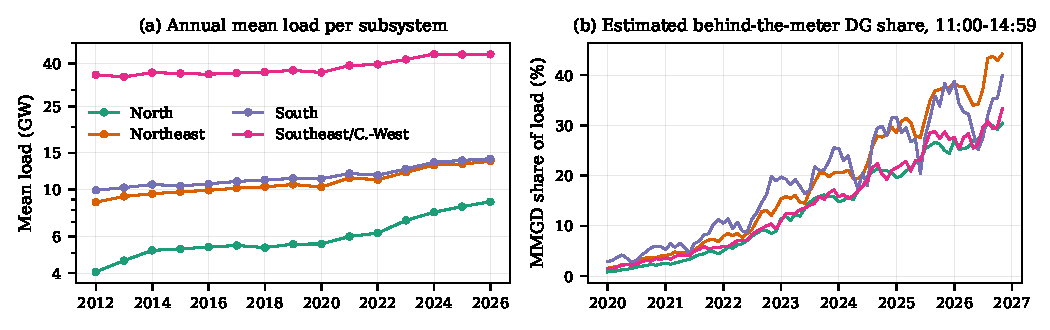
\includegraphics[width=\textwidth]{figures/fig_data.pdf}
\caption{(a) Annual mean hourly load of the four SIN subsystems (log scale; 2026 up to November 4). (b) Monthly mean share of the verified global load supplied by behind-the-meter distributed generation (MMGD) between 11:00 and 14:59, as estimated by ONS.}
\label{fig:data}
\end{figure*}

\begin{figure*}[!t]
\centering
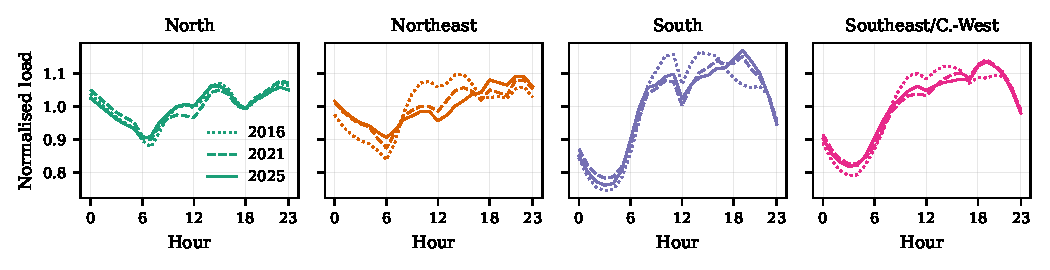
\includegraphics[width=\textwidth]{figures/fig_profiles.pdf}
\caption{Average weekday load profile, normalised by its daily mean, for 2016, 2021 and 2025.}
\label{fig:profiles}
\end{figure*}

\section{Methodology}
\label{sec:method}

\subsection{Forecasting Task and Information Set}
Let $y_{d,h}$ denote the load of a subsystem on day $d$ and hour $h\in\{0,\dots,23\}$. The task is to forecast the 24 values $\{y_{d,h}\}_{h=0}^{23}$ of the target day $d$ from information available at the issuance time, which we set to 12:00 of day $d-1$, consistent with the preparation of the daily operation programming. Allowing for data-collection latency, the most recent observation available at issuance is $y_{d-1,10}$ (the hour starting at 10:00). Hence, the forecast horizon ranges from 14 to 37 hours ahead and the most recent \emph{complete} day is $d-2$. This information set is stricter than the common simplification of using all of day $d-1$, and it guarantees that no model uses information unavailable to an operator.

\subsection{Level Normalisation}
Fig.~\ref{fig:data} shows strong trends, and tree-based models cannot extrapolate beyond the range of their training targets. We therefore divide the target and every load-valued input of day $d$ by the scale
\begin{equation}
s_d=\frac{1}{7\cdot 24}\sum_{k=2}^{8}\sum_{h=0}^{23} y_{d-k,h},
\label{eq:scale}
\end{equation}
the mean load of the seven most recent complete days. Models learn the normalised profile $\tilde y_{d,h}=y_{d,h}/s_d$ and forecasts are mapped back by multiplying by $s_d$. The effect of this choice is assessed in Section~\ref{sec:res_ablation}.

\subsection{Features}
All models share the same day-level input vector, built only from the information set above (Table~\ref{tab:features}): the normalised profiles of days $d-2$, $d-7$, and $d-14$ (24 values each); the observed hours 0--10 of day $d-1$; mean levels of the mornings of days $d-1$, $d-2$, and $d-8$; a weekly trend ratio; and calendar information. Calendar features comprise the day type (Monday to Sunday, or holiday), indicators for national holidays (including Good Friday, Corpus Christi, and the national Black Consciousness Day from 2024~\cite{lei14759}), Carnival Monday and Tuesday, Ash Wednesday, Christmas and New Year's eves, bridge days, and the year-end period (December~26 to January~6), indicators of whether the lagged days $d-1$, $d-2$, and $d-7$ were non-working days, and two pairs of annual Fourier terms. Holiday dates were generated programmatically from the Easter date and the national calendar; regional holidays are not modelled.

\begin{table}[!t]
\caption{Input features for target day $d$ (load features are divided by $s_d$).}
\label{tab:features}
\centering
\setlength{\tabcolsep}{3pt}
\begin{tabular}{p{0.34\columnwidth}p{0.56\columnwidth}}
\toprule
Group & Description \\
\midrule
Lagged profiles & $\tilde y_{d-2,h}$, $\tilde y_{d-7,h}$, $\tilde y_{d-14,h}$, $h=0,\dots,23$ \\
Same-day-before & $\tilde y_{d-1,h}$, $h=0,\dots,10$ \\
Levels & mean of hours 0--10 on $d-1$, $d-2$, $d-8$; ratio of the last two weekly means \\
Calendar (target day) & day type, holiday, Carnival, Ash Wednesday, eves, bridge day, year-end period, annual Fourier terms ($k=1,2$) \\
Calendar (lags) & non-working-day flags for $d-1$, $d-2$, $d-7$ \\
\bottomrule
\end{tabular}
\end{table}

\subsection{Models}
\subsubsection{Seasonal naive baselines}
SN7 uses the same hour one week earlier, $\hat y_{d,h}=y_{d-7,h}$. SN-DT uses the most recent day of the same type, i.e., $d-2$ for Wednesday to Friday when $d-2$ is a working day, and $d-7$ otherwise.

\subsubsection{ARX}
Following the LEAR philosophy~\cite{lago2021benchmark,ziel2018multivariate}, ARX consists of 24 hour-specific linear autoregressive models with exogenous calendar inputs, estimated jointly as a multi-output ridge regression on standardised inputs. The ridge penalty $\lambda$ is the only hyper-parameter.

\subsubsection{GBM}
A single global LightGBM model~\cite{ke2017lightgbm} is fitted on all (day, hour) pairs, with the hour of day and the day type as categorical inputs, and the hour-specific lags ($\tilde y_{d-2,h}$, $\tilde y_{d-7,h}$, $\tilde y_{d-14,h}$, $\tilde y_{d-1,h}$ when observed, and $\tilde y_{d-1,10}$) together with the level and calendar features. Missing inputs are handled natively.

\subsubsection{MLP}
A feed-forward neural network with ReLU activations maps the standardised day-level input vector to the 24 standardised outputs, trained with Adam and early stopping on the last 10\% of the training days; the forecast is the average of three networks with different random initialisations~\cite{pedregosa2011sklearn}.

\subsubsection{ENS}
The ensemble is the simple average of the ARX, GBM, and MLP forecasts, a combination scheme that is known to be hard to beat~\cite{petropoulos2022forecasting}.

\subsection{Probabilistic Forecasts}
We compare three ways of producing quantiles at levels $\tau\in\{0.05,0.10,0.25,0.50,0.75,0.90,0.95\}$:
(i) \emph{QGBM}, a LightGBM model per quantile with the pinball loss~\cite{koenker1978quantiles}, with quantile crossing removed by sorting;
(ii) \emph{EQR}, which adds to the ENS point forecast the empirical quantiles of its relative errors $e_{k,h}=y_{k,h}/\hat y_{k,h}-1$ over a rolling window of the last $W$ days with known outcomes ($k\le d-2$), computed separately for each hour, i.e., a split-conformal construction~\cite{vovk2022alrw}; and
(iii) \emph{ACI}, which applies adaptive conformal inference~\cite{gibbs2021aci} on top of EQR intervals: for a target miscoverage $\alpha$, the level used at day $d$ is updated as $\alpha_{d}=\alpha_{d-1}+\gamma(\alpha-\mathrm{err}_{d-2})$, where $\mathrm{err}_{d-2}$ is the fraction of hours of day $d-2$ outside the interval issued for that day, reflecting the delayed feedback of the operational setting. The window $W$ and step $\gamma$ were selected on the second half of 2023.

\subsection{Evaluation Protocol}
\label{sec:protocol}
All experiments use rolling-origin evaluation~\cite{bergmeir2012cv}: at each refitting date $t_0$, a model is fitted on the days in the calibration window ending at $t_0-2$ and used to forecast every day until the next refitting date. Unless stated otherwise, the calibration window is three years and models are refitted weekly. Hyper-parameters were selected once, on 2023 (validation year), using monthly refits, and kept fixed: the grids were $\lambda\in\{0.3,1,3,10,30,100,300\}$ for ARX; learning rate $\{0.03,0.06\}$, number of leaves $\{15,31,63\}$, number of trees $\{400,800\}$, and minimum leaf size $\{20,80\}$ for GBM; and hidden layers $\{(64),(128,64),(256,128)\}$ with $L_2$ penalty $\{10^{-4},\dots,10^{-1}\}$ for the MLP (the selected values are listed in Table~\ref{tab:hyper}). The test period is January~1, 2024 to November~4, 2026 (1,039 days, about 100{,}000 hourly forecasts across the four subsystems), which was never used for any modelling decision.

Point accuracy is measured by the mean absolute percentage error (MAPE) and the root mean squared error (RMSE)~\cite{hyndman2006accuracy}; MAPE is meaningful here because loads are far from zero. Differences in accuracy are tested with the one-sided DM test~\cite{diebold1995dm} with the Harvey--Leybourne--Newbold correction~\cite{harvey1997hln}, applied to the daily average of the hourly absolute percentage errors (the multivariate DM variant~\cite{ziel2018multivariate}), and $p$-values are adjusted for multiple comparisons with the Holm procedure~\cite{holm1979}. Probabilistic forecasts are evaluated by the empirical coverage and mean width of the 80\% and 90\% central intervals, the Winkler score~\cite{winkler1972interval}, and the average pinball loss over the seven quantiles~\cite{gneiting2007scoring}, all expressed relative to the mean load.

\begin{table}[!t]
\caption{Hyper-parameters selected on the 2023 validation year.}
\label{tab:hyper}
\centering
\setlength{\tabcolsep}{4pt}
\begin{tabular}{lp{0.62\columnwidth}}
\toprule
Model & Selected configuration \\
\midrule
ARX & ridge penalty $\lambda=10$ \\
GBM & learning rate 0.03, 63 leaves, 800 trees, minimum leaf size 20 \\
MLP & one hidden layer of 64 units, $L_2$ penalty $10^{-1}$, 3 seeds \\
QGBM & same as GBM, one model per quantile \\
EQR / ACI & window $W$ and step $\gamma$ in Table~\ref{tab:prob} \\
\bottomrule
\end{tabular}
\end{table}

\subsection{Comparison With the Official Forecast}
\label{sec:protocol_ons}
For the head-to-head comparison with the operator, the models are fitted on the verified global load, the quantity forecast by ONS, instead of the hourly curve. Because this series starts in 2020, an expanding window starting on January~1, 2020 is used, with weekly refits and the same information set, features, and hyper-parameters as above. The official forecast is taken as published, and the comparison is restricted to the days of the test period for which the official forecast is complete for all 24 hours (\NdaysONS{} days per subsystem). We do not know the exact cut-off time of the data used to produce the official forecast; since the daily programming is prepared on day $d-1$, our issuance time of 12:00 on $d-1$ with data up to 10:59 is unlikely to give the models an information advantage, an issue discussed in Section~\ref{sec:discussion}.

\section{Results}
\label{sec:results}

\subsection{Model Comparison}
\label{sec:res_main}
Table~\ref{tab:e1} reports the test-period accuracy of all models in the reference setting (three-year window, weekly refits). All learned models reduce the mean MAPE of the best seasonal naive benchmark (SN-DT, 4.44\%) by 33--40\%, and the ranking is remarkably stable across subsystems. The linear ARX model is the most accurate individual model, with a mean MAPE of 2.70\%, followed by the MLP (2.76\%) and the GBM (2.96\%). The simple ensemble ENS is the best model in all subsystems in terms of MAPE (2.66\% on average) and in three of the four in terms of RMSE. Errors are lowest in the North and Northeast (about 2\%) and highest in the South (about 4\%), where the load is the most temperature sensitive and where cold fronts and heat waves cause large day-to-day changes that a weather-free model cannot anticipate.

The DM tests (Table~\ref{tab:dm}) confirm that these differences are statistically significant: after the Holm correction, ARX is significantly more accurate than GBM in all four subsystems and than the MLP in three, and ENS is significantly more accurate than every individual model in at least two subsystems (than GBM and the MLP in all four). No model is significantly more accurate than ENS in any subsystem. That a regularised linear model beats a tuned gradient boosting model contrasts with the success of tree ensembles in retail and tabular competitions~\cite{makridakis2022m5,grinsztajn2022tabular}, but is consistent with the electricity price forecasting literature~\cite{lago2021benchmark}: with a strongly autoregressive target and smooth calendar effects, the 24 hour-specific linear models already capture most of the predictable structure, whereas the global tree model must learn the hour interactions from data. A hybrid in which a GBM learned the residuals of ARX was also evaluated on the validation year, but it did not improve on ARX (MAPE 2.68\% versus 2.65\%) and was discarded.

Fig.~\ref{fig:err}(a) shows that the error of every model peaks between 12:00 and 15:00 and is lowest overnight. This is the period in which behind-the-meter PV output, and thus the weather, has the largest effect on the load seen by the operator. Fig.~\ref{fig:err}(b) shows a clear seasonal pattern, with the largest errors from November to February (3.0--3.5\% averaged over subsystems), when convective rain and heat waves make both the cooling demand and the PV output volatile, and the smallest errors in July and August (about 2.1\%), during the dry austral winter; there is no upward trend over the test period.

\begin{table*}[!t]
\caption{Test-period accuracy (January 2024 -- November 2026) in the reference setting: MAPE (\%) and RMSE (MW) per subsystem, and MAPE averaged over subsystems. Best value per column in bold.}
\label{tab:e1}
\centering
\begin{tabular}{lccccccccc}
\toprule
& \multicolumn{2}{c}{North} & \multicolumn{2}{c}{Northeast} & \multicolumn{2}{c}{South} & \multicolumn{2}{c}{Southeast/C.-West} & All \\
\cmidrule(lr){2-3}\cmidrule(lr){4-5}\cmidrule(lr){6-7}\cmidrule(lr){8-9}\cmidrule(lr){10-10}
Model & MAPE & RMSE & MAPE & RMSE & MAPE & RMSE & MAPE & RMSE & MAPE \\
\midrule
\tabinput{tables/tab_e1.tex}
\bottomrule
\end{tabular}
\end{table*}

\begin{table}[!t]
\caption{Number of subsystems (out of four) in which the row model is significantly more accurate than the column model (one-sided DM test on daily MAPE, Holm-adjusted $p<0.05$).}
\label{tab:dm}
\centering
\setlength{\tabcolsep}{4pt}
\begin{tabular}{lcccccc}
\toprule
& SN7 & SNDT & ARX & GBM & MLP & ENS \\
\midrule
\tabinput{tables/tab_dm.tex}
\bottomrule
\end{tabular}
\end{table}

\begin{figure*}[!t]
\centering
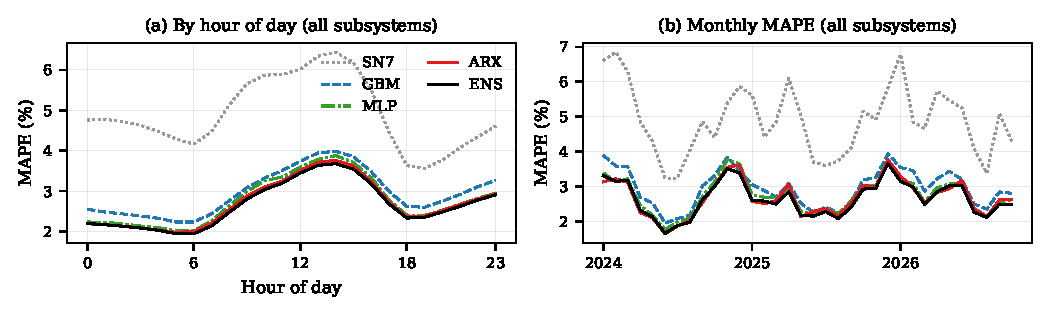
\includegraphics[width=\textwidth]{figures/fig_err_hour_month.pdf}
\caption{Test-period MAPE in the reference setting, averaged over the four subsystems: (a) by hour of the target day; (b) by month.}
\label{fig:err}
\end{figure*}

\subsection{Calibration Window and Refitting Frequency}
\label{sec:res_window}
Table~\ref{tab:e2} reports the mean MAPE of ARX and GBM for calibration windows from one year to the full history and refitting frequencies from daily to yearly. Two findings stand out. First, the refitting frequency matters much less than expected under drift: for ARX, moving from daily to yearly refits increases the MAPE by at most 0.06 percentage points (pp) for windows of two years or more, and for GBM the differences between refitting frequencies are at most 0.03~pp for every window. With level normalisation (Section~\ref{sec:method}), the slow growth of demand is absorbed by the scale $s_d$, so a model fitted a year earlier remains valid for the shape of the profile. Only ARX with a one-year window is sensitive to the refitting frequency (2.85\% with daily and 3.09\% with yearly refits), because a model fitted on a single year has seen each calendar situation only once. Second, the calibration window length matters more: one-year windows are clearly worse (ARX 2.85--3.09\%, GBM 3.23--3.25\%), and the accuracy improves up to five years for ARX (2.67\%) and up to the full history for GBM (2.83\%). Very long windows thus do not hurt, even though the load profile changed substantially over the period (Fig.~\ref{fig:profiles}): the annual Fourier terms, the lagged profiles, and the normalisation let the models represent recent profiles while benefiting from more examples of rare days, such as holidays. Averaging forecasts across windows, which is beneficial in price forecasting~\cite{hubicka2019windows,marcjasz2018windows}, brings no gain here: the average of the six weekly ARX forecasts reaches 2.67\%, equal to the best single window, and the average of the six monthly GBM forecasts 2.84\%, versus 2.83\% for the expanding window alone.

\begin{table}[!t]
\caption{Mean test MAPE (\%) over the four subsystems as a function of the calibration window and the refitting frequency (D: daily, W: weekly, M: monthly, Q: quarterly, Y: yearly). Weekly GBM refits were run only for 1- and 3-year windows. Best value per model in bold.}
\label{tab:e2}
\centering
\setlength{\tabcolsep}{2.6pt}
\begin{tabular}{lccccc|cccc}
\toprule
& \multicolumn{5}{c|}{ARX} & \multicolumn{4}{c}{GBM} \\
Window & D & W & M & Q & Y & W & M & Q & Y \\
\midrule
\tabinput{tables/tab_e2.tex}
\bottomrule
\end{tabular}
\end{table}

\subsection{Ablations}
\label{sec:res_ablation}
Table~\ref{tab:ablation} isolates the contribution of three design choices. Level normalisation is decisive for the tree model: without it, the GBM MAPE increases from 2.96\% to 3.23\%, and with an expanding window it is 3.25\% without normalisation versus 2.83\% with it (Table~\ref{tab:e2}), because the trees cannot produce values outside the range of past targets, which a growing load continuously exceeds. For ARX the normalisation is neutral (2.70\% in both cases), as expected for a linear model, and for the MLP it brings a small improvement. The special-day features reduce the MAPE of ARX by 0.24~pp and of GBM by 0.21~pp; although such days are only about 7\% of the test period, their errors are large enough to affect the overall averages (Section~\ref{sec:res_special}). The observations of the morning of day $d-1$ are the most valuable input of the tree model (without them, the GBM MAPE increases by 0.54~pp, and by 0.82~pp in the SE), and they reduce the ARX error by 0.19~pp: even 14 hours before the target day begins, the most recent load level carries information that the complete day $d-2$ does not.

\begin{table}[!t]
\caption{Ablations: mean test MAPE (\%) over the four subsystems in the reference setting.}
\label{tab:ablation}
\centering
\setlength{\tabcolsep}{3pt}
\begin{tabular}{p{0.56\columnwidth}ccc}
\toprule
Variant & ARX & GBM & MLP \\
\midrule
\tabinput{tables/tab_ablation.tex}
\bottomrule
\end{tabular}
\end{table}

\subsection{Special Days}
\label{sec:res_special}
Table~\ref{tab:daytype} breaks down the error by day type. National holidays, Carnival, Christmas and New Year's eves, and Ash Wednesday have errors 1.2--2 times those of regular weekdays for the learned models, and up to 2.3 times for the seasonal naive benchmark. Two patterns are worth noting. First, bridge days, which are not official holidays but on which many businesses close, are forecast almost as accurately as regular weekdays once they are flagged, showing that the programmatic calendar captures most of their effect. Second, different models are best on different special days, which is one reason why the ensemble is more robust than any single model; with only 3--30 occurrences of each type in the test period, however, these differences are not statistically conclusive. Days of the year-end period (December 26 to January 6), in which industrial activity is reduced, remain about 40\% harder than regular weekdays.

\begin{table}[!t]
\caption{Test MAPE (\%) by day type, averaged over the four subsystems ($n$: number of test days).}
\label{tab:daytype}
\centering
\setlength{\tabcolsep}{3pt}
\begin{tabular}{lcccccc}
\toprule
Day type & $n$ & SN7 & ARX & GBM & MLP & ENS \\
\midrule
\tabinput{tables/tab_daytype.tex}
\bottomrule
\end{tabular}
\end{table}

\subsection{Probabilistic Forecasts}
\label{sec:res_prob}
Table~\ref{tab:prob} compares the three probabilistic methods. On the validation period, the selected EQR window was $W=56$ days and the selected ACI step was $\gamma=0.005$. The quantile GBM is severely overconfident on the test period: its nominal 80\% and 90\% intervals cover only 53\% and 69\% of the observations. The quantiles are learned from in-sample fits, whose residuals are much smaller than the out-of-sample errors of a flexible model; flexible quantile regressors have no finite-sample calibration guarantee, which is precisely what motivated conformalised quantile regression~\cite{romano2019cqr}. The empirical relative-error quantiles of EQR, which are computed from genuine out-of-sample errors, are much better calibrated (77\% and 87\%) and also have a 16\% lower pinball loss than QGBM. ACI closes the remaining gap: with a small step, it attains 80.3\% and 90.1\% coverage, at the cost of intervals that are 9--15\% wider than those of EQR, and with a Winkler score very close to that of EQR.

Fig.~\ref{fig:cov} shows that the calibration of all methods varies over time. EQR coverage drops below 80\% during episodes in which the error distribution changes faster than its 56-day window can follow, mostly between September and December, when the transition from the dry winter to the hot season changes the level and the volatility of the errors, especially in the S and SE subsystems. ACI raises its intervals after such episodes and recovers the nominal coverage within a few weeks, but, because the feedback is delayed by two days and the step is small, it cannot prevent short-lived drops in coverage.

\begin{table}[!t]
\caption{Probabilistic forecasts on the test period, averaged over the four subsystems: coverage (Cov., \%), mean width (\% of mean load), and Winkler score (Wink., \% of mean load) of the central 80\% and 90\% prediction intervals, and mean pinball loss over seven quantiles (\% of mean load).}
\label{tab:prob}
\centering
\setlength{\tabcolsep}{2.8pt}
\begin{tabular}{lccccccc}
\toprule
& \multicolumn{3}{c}{80\% interval} & \multicolumn{3}{c}{90\% interval} & \\
\cmidrule(lr){2-4}\cmidrule(lr){5-7}
Method & Cov. & Width & Wink. & Cov. & Width & Wink. & Pinball \\
\midrule
\tabinput{tables/tab_prob.tex}
\bottomrule
\end{tabular}
\end{table}

\begin{figure}[!t]
\centering
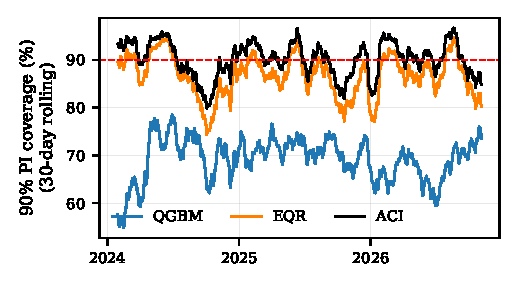
\includegraphics[width=\columnwidth]{figures/fig_coverage.pdf}
\caption{Coverage of the nominal 90\% prediction intervals over the test period (30-day rolling mean, averaged over the four subsystems).}
\label{fig:cov}
\end{figure}

\subsection{Comparison With the Official Forecast}
\label{sec:res_ons}
Table~\ref{tab:e6} compares the models fitted on the verified global load with the official ONS day-ahead forecast over the \NdaysONS{} common test days. ENS is more accurate than the official forecast in all four subsystems: its MAPE is 25\% lower in the North (1.96\% versus 2.62\%), 28\% lower in the Northeast (1.96\% versus 2.71\%), 9\% lower in the South (3.57\% versus 3.92\%), and 3\% lower in the Southeast/Center-West (2.26\% versus 2.33\%); on average, the reduction is 16\% (2.44\% versus 2.90\%). The improvement is significant according to the DM test in the North, Northeast, and South ($p<0.001$), but not in the Southeast/Center-West ($p=0.10$), where the official forecast also has a slightly lower RMSE. ARX and the MLP individually lead to the same conclusions, whereas GBM is significantly more accurate than the official forecast in the North and Northeast but significantly less accurate in the Southeast/Center-West. ENS gives the lower daily MAPE on 73\%, 70\%, 60\%, and 56\% of the days in the N, NE, S, and SE subsystems, respectively.

The error profile by hour (Fig.~\ref{fig:ons_hour}) explains these results. In the North and Northeast, the error of the official forecast rises sharply between 07:00 and 16:00, and between 10:00 and 14:00 it is 1.8 times the error of ENS in the North (4.3\% versus 2.4\%) and 1.5 times in the Northeast (3.8\% versus 2.6\%), whereas the gap is much smaller at night. In the South and Southeast/Center-West, the official forecast is slightly more accurate in the afternoon (14:00--17:00) and late evening, i.e., at the hours in which temperature drives the load, and ENS is more accurate at night and in the morning.

The midday errors of the official forecast are not random: they are a growing systematic under-forecast. Between 10:00 and 14:00, the mean relative bias of the official forecast went from $-2.8\%$, $-0.8\%$, $-0.5\%$, and $-1.0\%$ in 2024 to $-3.9\%$, $-3.0\%$, $-2.4\%$, and $-2.3\%$ in 2026 in the N, NE, S, and SE subsystems, respectively, whereas the bias of ENS stayed within $\pm1.3\%$ in every year and subsystem. Fig.~\ref{fig:ons_bias} shows the monthly midday bias together with the share of the global load supplied by MMGD: the official forecast's bias deepens as this share grows, with monthly correlations between $-0.31$ (N) and $-0.54$ (NE and S). Consistent with this, the annual MAPE of the official forecast increased from 2024 to 2026 in all subsystems (e.g., from 2.28\% to 2.83\% in the North and from 2.31\% to 2.93\% in the Northeast), whereas that of ENS remained stable (1.94\% to 1.97\% and 1.85\% to 2.04\%, respectively).

From July 2026 onwards, the midday bias of the official forecast became much smaller in all subsystems (Fig.~\ref{fig:ons_bias}), which suggests a revision of the operator's procedure. Even in these last four months (127 days), however, ENS remained significantly more accurate in the North (1.58\% versus 1.93\%), Northeast (1.77\% versus 2.24\%), and South (2.95\% versus 3.63\%), and statistically equivalent in the Southeast/Center-West (2.41\% versus 2.35\%), so the midday bias is the main, but not the only, source of the difference.

Because the exact data cut-off of the official forecast is not published, we repeated the comparison with an ARX model that does not use any observation of day $d-1$, i.e., with data only up to the end of day $d-2$. This model remains significantly more accurate than the official forecast in the North (2.07\% versus 2.62\%) and the Northeast (2.14\% versus 2.71\%), is statistically indistinguishable in the South (3.98\% versus 3.92\%), and is significantly less accurate in the Southeast/Center-West (2.54\% versus 2.33\%). The advantage in the North and Northeast therefore does not depend on the most recent observations, whereas in the two southern subsystems the information of the morning of day $d-1$ is what makes a weather-free model competitive.

Finally, the two forecasts are partly complementary. An equal-weight average of ENS and the official forecast, which requires no estimation, reduces the MAPE further in the South (3.38\%) and the Southeast/Center-West (2.07\%), the subsystems where the official forecast is competitive and presumably benefits from weather information, but not in the North and Northeast (2.11\% and 2.12\%), where the official forecast's midday bias dominates.

\begin{table*}[!t]
\caption{Comparison with the official ONS day-ahead forecast on the verified global load (common test days, January 2024 -- November 2026): MAPE (\%) and RMSE (MW). $^{+}$/$^{-}$: model significantly more/less accurate than the official forecast (one-sided DM test on daily MAPE, $p<0.05$). Best value per column in bold.}
\label{tab:e6}
\centering
\begin{tabular}{lccccccccc}
\toprule
& \multicolumn{2}{c}{North} & \multicolumn{2}{c}{Northeast} & \multicolumn{2}{c}{South} & \multicolumn{2}{c}{Southeast/C.-West} & All \\
\cmidrule(lr){2-3}\cmidrule(lr){4-5}\cmidrule(lr){6-7}\cmidrule(lr){8-9}\cmidrule(lr){10-10}
Forecast & MAPE & RMSE & MAPE & RMSE & MAPE & RMSE & MAPE & RMSE & MAPE \\
\midrule
\tabinput{tables/tab_e6.tex}
\bottomrule
\end{tabular}
\end{table*}

\begin{figure*}[!t]
\centering
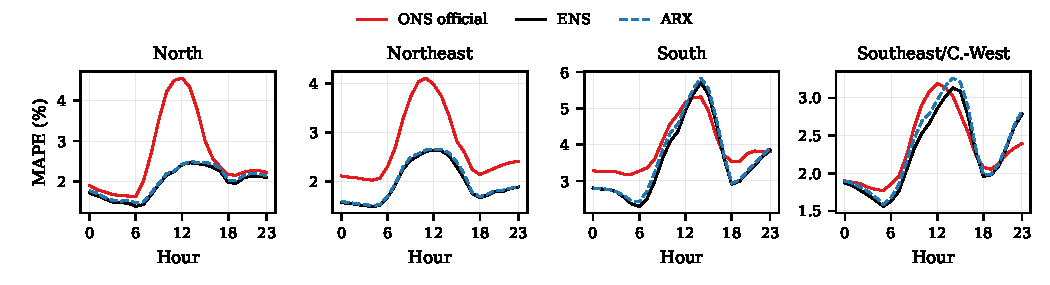
\includegraphics[width=\textwidth]{figures/fig_ons_hour.pdf}
\caption{MAPE by hour of the target day of the official ONS forecast, ENS, and ARX on the verified global load (common test days).}
\label{fig:ons_hour}
\end{figure*}

\begin{figure*}[!t]
\centering
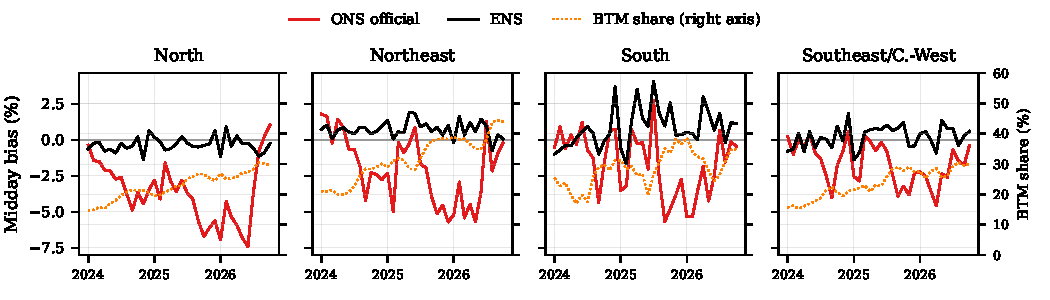
\includegraphics[width=\textwidth]{figures/fig_ons_bias.pdf}
\caption{Monthly mean relative bias (forecast minus verified, \% of verified load) between 10:00 and 14:59 of the official ONS forecast and of ENS (left axes), and share of the verified global load supplied by behind-the-meter MMGD in the same hours (dotted, right axes).}
\label{fig:ons_bias}
\end{figure*}

\section{Discussion}
\label{sec:discussion}

\subsection{Why Can Weather-Free Models Beat an Operational Forecast?}
The official forecast of ONS uses weather forecasts and the experience of the operator's forecasting staff, information that our models do not have. Its lower accuracy in three of the four subsystems is therefore not a statement that simple models are better forecasters in general. Our results point to a specific mechanism. The official forecast's error is concentrated in the hours of PV generation, takes the form of an under-forecast of the global load, and grows over time together with the share of behind-the-meter MMGD (Fig.~\ref{fig:ons_bias}). The global load is the sum of the load measured at the transmission level and the estimated MMGD output; a forecast built on a component that does not keep up with the fast-growing installed MMGD capacity, or on profiles learned when this capacity was smaller, would under-forecast the midday global load in exactly this way. The models in this study learn the target directly from the most recent verified data: the level normalisation and the lagged profiles of days $d-2$, $d-7$, and $d-14$ make them adapt to the changing shape of the profile within a few weeks, without any explicit representation of PV. The fact that ENS shows no bias trend over almost three years, in all subsystems, supports this explanation, as does the reduction of the official forecast's bias from July 2026 onwards. That ENS remained more accurate after this reduction indicates that the timely use of the most recent load observations is a second, independent source of advantage. In the South and Southeast/Center-West, where the official forecast is competitive and more accurate in the afternoon, the weather information it contains is valuable, as also shown by the gains of the simple combination of the two forecasts.

These findings are relevant beyond Brazil. Many systems are going through a similar transition, and operators often forecast the load seen at the transmission level, net of behind-the-meter PV, or reconstruct the gross load with an estimate of PV output. In both cases, the forecast must keep up with installed capacity that changes every month. Our results suggest three simple practices for operators and forecasters: monitoring the bias of the forecast by hour of the day, not only its overall accuracy; maintaining at least one data-driven benchmark fitted on recent data, which is cheap and acts as an early-warning signal; and combining it with the operational forecast, which in our case reduced the error in the two subsystems where the official forecast is strongest.

\subsection{Practical Recommendations for Model Design}
For practitioners building day-ahead load models under drift, the experiments lead to concrete recommendations. (i) Normalise the target and the load inputs by a recent level before fitting tree-based models; without this, tree ensembles cannot follow a growing load, and the advantage of weekly refits or long windows is lost. (ii) Use calibration windows of three years or more: shorter windows cost more accuracy than any change in the refitting frequency. (iii) Frequent refitting is not necessary when the level is normalised: for windows of two years or more, monthly or even quarterly refits are within 0.05~pp of daily refits, which reduces the computational cost, especially for neural and tree models. (iv) Strong linear benchmarks should always be reported: ARX, which takes seconds to fit, was more accurate than a tuned GBM and an MLP, and the gain of the ensemble over ARX was small (0.04~pp) although significant in two subsystems. (v) For prediction intervals, empirical quantiles of recent out-of-sample errors are a better starting point than quantile regression with flexible models, and adaptive conformal inference with the operational delay restores the nominal coverage at little cost.

\subsection{Limitations}
This study has limitations that also indicate directions for further work. First, the models do not use weather forecasts. Historical numerical weather predictions for Brazil at the required resolution are not openly available for the whole period, and reanalysis data would give the models information unavailable at forecast time. Adding operational weather forecasts would most likely reduce the errors in the afternoon and in the South, where the official forecast is competitive. The weather-free setting, however, makes the comparison conservative with respect to our models. Second, the exact data cut-off of the official forecast is not documented. We used an issuance time of 12:00 on day $d-1$, consistent with the preparation of the daily operation programming, and showed that the conclusions for the North and Northeast hold even without observations of day $d-1$. Third, the verified global load contains an estimate of MMGD output produced by ONS, so the target itself is partly modelled. This affects the official forecast and our models in the same way, but the comparison should be interpreted as accuracy with respect to the operator's own verified series. Fourth, regional and municipal holidays, which matter in particular for the smaller subsystems, are not modelled. Finally, the evaluation covers one system. The mechanism we identify is general, but replicating the comparison with the data of other operators that publish their official forecasts, such as those of Australia or Europe, would confirm whether the size of the effect is similar elsewhere.

\section{Conclusion}
\label{sec:conclusion}
This paper presented an open and fully reproducible benchmark for day-ahead hourly load forecasting of the four subsystems of the Brazilian interconnected system, built exclusively from public operator data and evaluated over almost three years with an operationally realistic information set. Linear ARX models, a gradient boosting model, a neural network, and their average were compared, and the best open models were evaluated against the official day-ahead forecast of the system operator.

The main findings are as follows. First, a simple average of ARX, GBM, and MLP forecasts, without any weather input, was 16\% more accurate than the official forecast on average (MAPE 2.44\% versus 2.90\%), with significant gains in three of the four subsystems. Second, the official forecast shows a systematic midday under-forecast that grew from 2024 to 2026 together with the share of behind-the-meter generation, whereas the open models remained nearly unbiased; this bias is the main source of the difference in accuracy, although the open models remained more accurate after the bias was reduced in mid-2026. Third, under drift, the calibration window length matters more than the refitting frequency, and level normalisation is essential for tree-based models. Fourth, adaptive conformal inference with delayed feedback produced calibrated prediction intervals, whereas quantile gradient boosting was strongly overconfident.

Future work will add operational weather forecasts, extend the comparison to other operators that publish their official forecasts, and study forecast combinations that explicitly correct the hour-specific bias of operational forecasts. The code and data pipeline are released so that the benchmark can be updated as new data are published.


\section*{Data and Code Availability}
All data used in this study are public and were obtained from the open-data portal and the load API of the Brazilian National System Operator (ONS)~\cite{ons_opendata,ons_apicarga}. The complete source code required to download the data, reproduce every experiment, and regenerate all tables and figures is available at \url{https://github.com/izialber/artigo-ieee}.

\section*{Acknowledgment}
The author thanks the Brazilian National System Operator (ONS) for making its operational data openly available.
In accordance with IEEE policy on the use of artificial-intelligence-generated content, the author discloses that an AI system (Claude, Anthropic) was used to assist in writing the software, running the experiments, and drafting and editing the manuscript text. All results were produced by the released code from public data, and the author reviewed the methodology, results, and text and takes full responsibility for the content of this article.

\bibliographystyle{IEEEtran}
\bibliography{references}

\begin{IEEEbiographynophoto}{IZIALBER OZANI FERNANDES MUNIZ}
is a graduate student in the Graduate Program in Production and Systems Engineering (PPPRO) at CEFET/RJ, Rio de Janeiro, Brazil. Research interests include energy forecasting, machine learning for power systems, and time-series analysis.
\end{IEEEbiographynophoto}

\EOD

\end{document}
